\chapter{Intent Change Estimation Based on Physical Interactions of an	Exoskeleton User}\label{chapter:BKF}

The IMM estimation framework presented previously is reactive, as it monitors signs of gait transition. For example, if the CoM trajectory after gait transition does not resemble library gaits, the IMM algorithm will misidentify the intended change until after it has been realized. However, anticipative intent inference is more desirable to time the assistance delivery appropriately and help the user realize their intended gait transition. Improper assistance timing may result in the robot resisting the user's actions, hampering HRI fluency. Intent may be anticipatively inferred by identifying early signs of a transition within the actions the user takes to realize their intent change. Actions indicative of intent change may be detected by monitoring the interactions the user has with the exoskeleton and the environment as well as their impact on other gait features. This pHRI may provide an earlier indicator of intent changes compared to CoM or joint motions, making it possible to anticipate user intent and provide assistance to the user to help realize the desired objective. 

Some currently available exoskeletons targeted towards people with iSCI use rudimentary methods to infer user intent for step initiation via basic pHRI. The HAL exoskeleton uses force sensors under the feet to detect weight transfer to initiate a step \cite{suzuki2007intention}, and the ReWalk system uses a combination of ground reaction force sensors and torso tilt \cite{goffer2012locomotion}. The work presented in this chapter applies pHRI-based estimation to infer the exoskeleton user's desire to change gait speed. As first principles do not apply to the decisions humans make to realize speed changes, the learning-based strategies are employed in the work detailed herein.

Learning-based strategies model gait patterns by forming data-driven relationships between the gait and sensor measurements. Lee et al. used a Convolutional Neural Network (CNN) to predictively estimate user intent in real time with low error rates \cite{lee2020image}. The CNN, which was trained using walking data from healthy individuals, uses measurements from various sensors such as electromyography (EMG), IMUs, and electrogoniometers to classify intent between level walking and ramp and stair ascent/descent. Thatte et al.~developed an estimator that uses a Gaussian Process (GP)-based Extended Kalman Filter \cite{thatte2019robust} to estimate the user's gait phase during stance to control a prosthetic leg. An intent recognition scheme for lower-limb prostheses \cite{young2013classifying} employed Linear Discriminant Analysis (LDA) to classify heel-strike and toe-off based on EMG and mechanical sensors onboard the prosthetic device. 

The intent detection methods described previously are targeted towards people using prostheses and identify a broad activity such as walking on flat ground, stair ascent/descent, or sitting/rising from a chair. While limited work exists for intent estimation for exoskeleton users, Gambon et al.~presented an algorithm \cite{Gambon20b} to identify instances where an exoskeleton user wanted to walk faster or slower than their nominal speed based on the Mahalanobis distance of the sensor measurements from the nominal trajectory. The work presented in this chapter outlines a method to identify an exoskeleton user's desire to change gait speed. 

The main contribution of this work is a new Bayesian estimation framework, termed the Buttressed Kalman Filter, that relies on a simple model to anticipate a user's intent to change speeds before it happens physically. Since ground contacts greatly influence the stability of legged locomotion, it was hypothesized that user intent will be reflected in the contacts chosen. As such, the work presented in this chapter explores exploiting changes in foot placement to infer the intended gait speed changes of an exoskeleton user. 

The footstep model emulates the trends in step length versus gait speed in uninjured individuals as an indicator of intent change. An additional model for RMS hip motor currents was used for individuals with iSCIs to capture the users' interaction with the exoskeleton and improve estimation accuracy. This framework was evaluated on the dataset of walking trials described in Section~\ref{sec:exoData}. The framework was able to estimate whether the user wants to speed up or slow down, and did so before the user realized the speed change.

The rest of this chapter is organized as follows. Section~\ref{sec:quantification} describes the choices made to quantify user intent using gait speed, and the relationship between gait speed and foot placement. Section~\ref{sec:BKF} details the two-stage estimation framework used to incorporate information gained from foot placement into the intent estimation problem. The performance of the estimation framework was evaluated on experimental data and is discussed in Section~\ref{sec:bkf_results}. Additional analysis to guide the improvement of estimator performance is described in Section~\ref{sec:add_analysis}. This analysis compares the benefits of increasing the number of gait features versus increasing model complexity. The chapter summary is provided in Section~\ref{sec:bkf_summary}. This chapter describes the results reported in a previous journal publication \cite{karulkar2021using}.

\section{Quantifying intent - Enabling estimation}\label{sec:quantification}
User intent is an abstract notion, so it must be quantified and inferred using a measurable quantity, and this quantification is a design choice. The intended gait speed was chosen to represent user intent, as the primary objective of the exoskeletons herein is gait rehabilitation. Estimating the gait speed of an individual may increase the possibility for finer control of the gait and also limit the need to train for multiple discrete scenarios. The state of the exoskeleton user CoM is represented in a vector 
\[
	\x = \begin{bmatrix}
		\mathbf{p}_{CoM} \\
		\mathbf{v}_{CoM}
	\end{bmatrix}
\] 
To capture intent, the state was extended to include the intended gait velocity $ z $ as a hidden state in an augmented state vector $ \q = [\x^{\top} ,z]^{\top} $. The gait velocity $ z $ only represents the forward speed in the sagittal plane. Velocity in the transverse\footnote{The transverse plane is the plane that divides the body into top and bottom parts. } plane (e.g., while turning) is neglected, as the exoskeleton restricts adduction/abduction of the legs. This state augmentation approach allows using the Kalman filter to directly estimate the intended gait speed. 

Previously performed studies of bipedal locomotion provided an idea of how changes in walking gaits correspond to transitions in user intent. These physical indicators include differences in CoM trajectories and foot placement, as illustrated in Fig.~\ref{fig:main_idea}. Ground contacts greatly influence the stability of legged locomotion, so it was hypothesized that intent will be reflected strongly in the user's choice of ground contacts through foot placement \cite{bhounsule2014foot}. Modulating foot placement while walking is an effective control mechanism to maintain stability \cite{hof2010balance,bhounsule2015control}, and it has been shown that velocity changes at MS influence foot placement at TD \cite{wang2014stepping,redfern1994model}. 
%
\begin{figure}
	\centering
	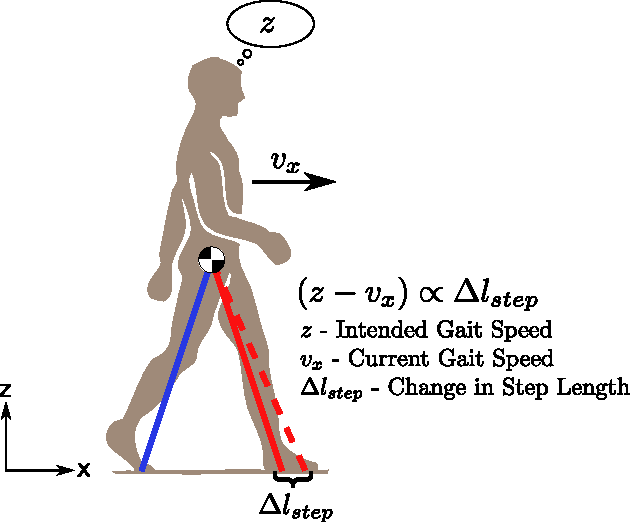
\includegraphics[width=0.6\linewidth]{main_idea_bkf}
	\caption{Change in intended velocity may be inferred from change in step length}\label{fig:main_idea}
\end{figure}

\subsection{Transitioning from a model-based to a data-driven approach}
The B-SLIP model may be used to adequately model steady-state walking, and foot placement was found to be critical in optimizing periodic gaits. The model, however, does not inherently capture the active changes required to change speed. Additionally, no first-principles apply to the actions humans take towards foot-placement as a function of the desired gait speed. These aspects were initially modeled by designing a controller for the B-SLIP model to emulate human motor control. With such a design, intent changes may be considered analogous to controller setpoint changes. Several theories try to explain human motor control, one of which says that the human sensorimotor system relies on optimal control \cite{todorov2004optimality,sylla2014assessing}. Therefore, we chose to assume the human motor controller to be a Linear Quadratic Regulator (LQR). The MS-to-MS Poincar\'e map was linearized about a periodic gait, and the linearized model was used to design a controller that minimized deviations from a specified gait. 

The dynamics of the B-SLIP model are nonlinear, and linearizing them about a single periodic gait results in a model valid for a very small portion of the gait, which rendered the controller unable to handle large speed changes. A derivative-free technique, i.e., the Unscented Transform \cite{manchester2016derivative}, was employed to generate a linear model. This technique required integrating dynamics backward in time, which was difficult to do for the hybrid dynamics of the B-SLIP model as the gait event timing cannot be fixed. Therefore, due to the lack of first principles that describe human choices to bring about intended gait changes, a data-driven approach was chosen to model the relationship between intended gait speed and foot placement.

\subsection{Relationship between foot placement and gait speed }
There is a correlation between step length and walking speed that can be exploited to infer changes in intended gait speed. People walking unassisted at lower velocities exhibit shorter step lengths, and an increase in velocity results in an increase in step length \cite{kuo2001simple,andriacchi1977walking}, as illustrated in Fig.~\ref{fig:step_change}. Such a velocity-step-length relationship can also be viewed as valid assuming that the walk ratio is roughly constant \cite{sekiya1997optimal}. 
%
\begin{figure}
	\centering
	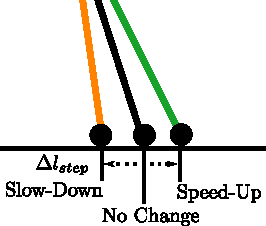
\includegraphics[width=0.35\linewidth]{step_change.pdf}
	\caption{Speed-up and slow-own increase and decrease the step length respectively}\label{fig:step_change}
\end{figure}
%
The walk ratio, defined as the ratio of the step length to cadence~\cite{rota2011walk}, is fairly invariant with respect to gait speeds for community ambulation, i.e.,~gait velocities greater than 0.8 m/s, despite age and terrain differences. It is affected when attention is divided between motor and cognitive tasks, i.e., dual-task walking \cite{bogen2018walk}. The walk ratio increases as speed decreases below community ambulation velocities \cite{murakami2017estimated} and is dependent on the nature and severity of injuries \cite{rota2011walk} during unassisted walking. In rehabilitation, the variability in the walk ratio may be reduced due to the stability provided by the exoskeleton structure and consistent timing of the exoskeleton assistance \cite{seo2015new}. While the effects of exoskeleton-assisted walking on the walk ratio remain open, this analysis suggests that it is reasonable to assume a constant walk ratio for the work herein.

\section{Framework to estimate desired gait speed}\label{sec:BKF}

It was assumed that intent changes made at the first MS are reflected in the placement of the foot at TD and then maintained as constant until the subsequent MS. As illustrated in Fig.~\ref{fig:step_stages}, a step is modeled as starting at MS, finalizing the placement of the leading foot at TD, and finishing at the next MS. Therefore, a twice-per-step strategy that relies on a simple model to exploit the relationship between velocity change and step length change was used to estimate intent at TD and MS. 

\subsection{Buttressed Kalman Filter}
\begin{figure}
	\centering
	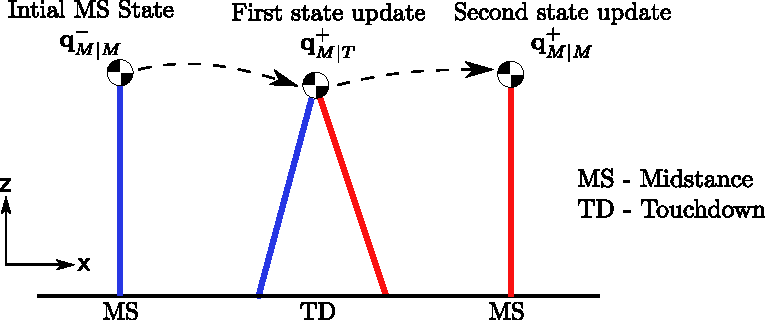
\includegraphics[width=0.8\linewidth]{step_stages.pdf}
	\caption{Two-stage estimation process}\label{fig:step_stages}
\end{figure}

A staged estimation scheme, as illustrated in Fig.~\ref{fig:block_diag}, was considered to infer intent changes using step length change information. The unit delay represents the passing of estimates as initial conditions for the next estimation cycle. In this scheme, footstep information at TD was first used to update the intent state for the initial MS. The position and velocity of the CoM were then corrected with a second update at the terminal MS of the step. A simple data-driven model of step length was used as a function of the velocity $ v_x $ at the MS prior to TD, desired velocity $ z $, and leg length $ l_{leg} $:
%
\begin{equation}
	l_{step} = [v_x\ (z-v_x)\ l_{leg}] \greekvec{\kappa} \label{eq:stepModel},
\end{equation}
where $ \greekvec{\kappa} $ is a vector containing regression coefficients and the model output is a scalar value in meters. This model takes into consideration the nominal step length as a function of leg length, the current velocity, and desired velocity.

\begin{figure}
	\centering
	\begin{overpic}[width=0.8\linewidth,percent]{block_diagram}
		\put(13,11){ \eqref{eq:sig_yy} - \eqref{eq:tdCovUp}}
		\put(48,11){\eqref{eq:model} - \eqref{eq:P_up}}
	\end{overpic}
%	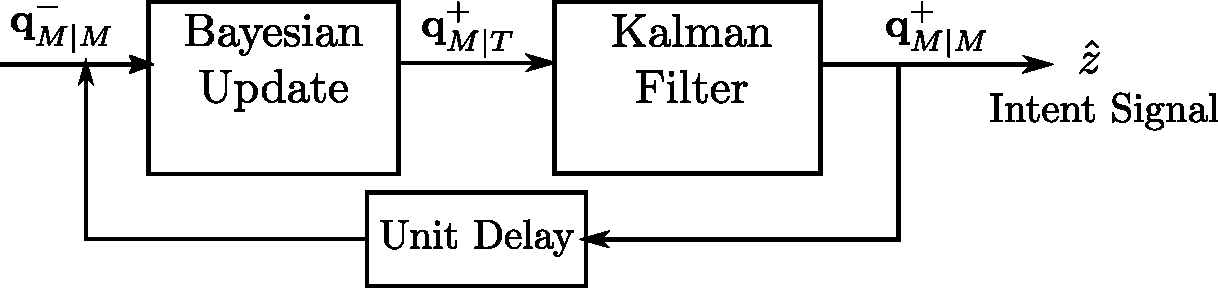
\includegraphics[width=0.7\linewidth]{block_diagram.pdf}
	\caption{Twice-per-step strategy to estimate user intent}\label{fig:block_diag}
\end{figure}

The step length model may be used as a measurement model in a Kalman filter framework to relate the intended gait speed to the measured step length. The estimator operates on the state $ \hat{\q} $ and its covariance $ \P $. In the following equations, the superscripts $ - $ and $ + $ denote pre-/post-update states, respectively, the subscripts $ M $ and $ T $ denote MS and TD, respectively, and the bar denotes the update location. For instance, $\hat{\q}_{M|T}^+ $ represents the state of the CoM at MS updated at TD. 

Predicted step length $ \hat{\y}_{T} $ was computed from \eqref{eq:stepModel} using the state estimate $ \hat{\q}_{M|M}^- $
\[
	\hat{\y}_{T} =  l_{step}(\hat{v}_x,\hat{z}, l_{leg})
\]
Since the footstep model is data-driven and may have inaccuracies, a process noise covariance $ \Q_{T} $ was added to the state estimate covariance $ \P^-_{M|M} $. Additionally, the estimated measurement covariance $ \Ssigma_{yy} $ was computed using the Jacobian of the measurement model $ \H_{T} $ and measurement covariance $ \R_{T} $ such that 
%
\begin{eqnarray}
	\H_{T} &=& \left. \frac{\partial \hat{\y}_{T}}{\partial \q}\right|_{\hat{\q}} \nonumber \\
	\Ssigma_{yy} &=& \H_{T} \left(\P^-_{M|M} + \Q_{T}\right) \H_{T}^{\top} + \R_{T} \label{eq:sig_yy}
\end{eqnarray}
%
The predicted step length was compared to the measured step length $ \tilde{\y}_{T} $, and the state at MS $ \hat{\q}_{M|M}^- $ and its covariance were updated using a Bayesian update
%
\begin{eqnarray}
	\hat{\q}_{M|T}^+ &=& \hat{\q}_{M|M}^- + \P^- \H_{T}^{\top} \Ssigma_{yy}^{-1} (\tilde{\y}_{T} - \hat{\y}_{T})  \label{eq:tdUp}\\
	\P^+_{M|T} &=& \P^-_{M|M} -\P^-_{M|M} \H_{T}^{\top} \Ssigma_{yy}^{-1} \H_{T} \P^-_{M|M} \label{eq:tdCovUp}
\end{eqnarray}

This update to the previous MS state using TD information then primes $ \hat{\q}_{M|T}^+ $ and $ \P^+_{M|T} $ to be used with a Kalman filter.	Simple dynamics are used to propagate this state and covariance to the next MS 
\begin{eqnarray}
			\hat{\q}_{M|T}^+ &\leftarrow& \D \hat{\q}_{M|T}^+ \label{eq:model}\\
			\P^+_{M|T} &\leftarrow& \D  \P^+_{M|T} \D^{\top} + \Q_{M} \label{eq:cov}
\end{eqnarray}
%
where $ \D = {\rm diag}([1 ,-1 ,1 ,1 ,-1 ,1 ,1]) $. These simple dynamics change the signs of the lateral position and velocity of the CoM to emulate the switching of the stance foot and allow for the application of a standard Kalman filter from MS to MS. It is assumed that the motion of the CoM is periodic with respect to the stance foot; however, since the CoM position is referenced from the stance foot, which changes step to step, the lateral position and velocity also change signs. 

The second update takes place at the next MS, with the stance foot switched. The outputs of \eqref{eq:model} and \eqref{eq:cov} are updated using a Kalman update 
\begin{eqnarray}
	\K &=& \P^+_{M|T} \H_{M}^{\top} \left(\H_{M} \P^+_{M|T} \H_{M}^{\top} + \R_{M}\right)^{-1}\\
	\hat{\q}_{M|M}^+ &=& \hat{\q}_{M|T}^+ + \K(\tilde{\y}_{M} - \H_{M} \hat{\q}_{M|T}^+) \\
	\P^+_{M|M} &=& (\I - \K \H_{M}) \P^+_{M|T} \label{eq:P_up}
\end{eqnarray}
where the measurement model Jacobian is $ \H_{M} = \I^{6\times7} $ since the measurements are $ \tilde{\y}_{M} = [\tilde{\p}_{CoM} ,\tilde{\v}_{CoM}]^{\top} $.

This approach varies from a conventional Kalman filter formulation, in that the information obtained at TD is used to update the prior distribution for the MS-to-MS estimator. As the dynamics-free Bayesian update reinforces the MS-to-MS Kalman filter, this estimation setup has been termed as a Buttressed Kalman Filter.

The estimator needs to send an output signal to the exoskeleton to inform its controller of changes in the user's intent. Since the representation of user intent was chosen to be the forward velocity, the change of $ \hat{z} $ from MS to MS represents the user's desire to change gait speed. The estimator uses a simple model to predict the step length, so it does not emulate the exact relationship between the velocity at MS and the ensuing step length. As a result, using the estimated value of the intended velocity is not a good indicator of intent, as this value may not match the measured values. However, the change of the intended velocity from MS to MS $ \Delta z $ is a better candidate for intent change indication. This quantity represents the expected ``acceleration" from MS to MS, so it can be considered to be a ``speed-up" signal when the rate is positive or a ``slow-down" signal when the rate is negative. Inferring intent as a ``speed-up" or ``slow-down" signal is consistent with the fundamentally abstract nature of intent as opposed to the concrete velocity value given by the estimator. This ability to capture continuous adjustments may result in finer control of the exoskeleton compared to discrete activity classification that is more commonly used.

\subsection{Simple model to relate intended velocity and foot placement}

The two main gait events to be identified for the estimator were MS and TD. For healthy individuals walking independently, the foot touchdown process starts with a heel strike, the ankle then undergoes plantarflexion, and the foot then rests flat on the ground. Plantarflexion is the motion of the foot about the ankle when it rotates away from the shank, and since the exoskeleton has no ankle mobility, the subject has to touch down with a nearly flat foot. This results in step lengths that are shorter than those observed in independent walking. Additionally, the subject walking in the exoskeleton used an ambulatory device such as a walker or crutches. Consequently, data from walking trials of subjects using the Ekso GT \cite{exoWalkerData} were used in the regression for the step length model shown in \eqref{eq:stepModel}. To perform the regression, the velocity at the subsequent MS was assumed to be the desired velocity. For example, suppose $ v_k $ was the forward velocity of the user at MS at time $ k $. The regression was set up such that $ l_{step,{k+1}} = [v_{k}\ (v_{k+1}-v_{k})\ l_{leg}] \greekvec{\kappa} $, where the subscript $ x $ has been omitted for conciseness, and the desired velocity was assumed as $ v^d = v_{k+1} $. This formulation provided insight into the step length, using future velocity data to provide a proxy for the intended velocity.

\section{Results with walking trial data}\label{sec:bkf_results}

The BKF was first evaluated on walking data from a subject without iSCI using the exoskeleton in free mode, and the results are described in Section~\ref{sec:ab_results}. The framework was then evaluated on data from a subject with an iSCI with the exoskeleton in adaptive mode, and the results are discussed in Section~\ref{sec:nab_results}.

\subsection{Subject without iSCI}\label{sec:ab_results}
The trial shown in this section was that of a subject without iSCI walking in free mode. In this mode, the exoskeleton provides constant assistance akin to gravity compensation to the user. The measurement used at TD was the step length, so the measurement vector was $ \tilde{\y}_{T} = [l_{step}] $. Measurements of all positions and velocities were available at MS, so $ \tilde{\y}_{M} = [\p_{CoM}^{\top} ,\v_{CoM}^{\top}]^{\top} $. The process noise covariance $ \Q $ and the measurement noise covariance $ \R $ were given by
\begin{eqnarray}
	\Q_M &=& {\rm diag}([1 ,1 ,1 ,1 ,1 ,1 ,10]) \times 10^{-4} \\
	\R_M &=& {\rm diag}([10^{4} ,10^{4} ,10^{4} ,10^{5} ,1 ,1]) \times 10^{-10} \\ % x y z vx vy vz at MS 
	\Q_T &=& 10^{-4} \\
	\R_T &=& 10^{-5} % xf at TD
\end{eqnarray}
where process noise covariances for positions and velocities are reported with units m\textsuperscript{2} and m\textsuperscript{2}/s\textsuperscript{2}, respectively.

\begin{figure}
	\centering
	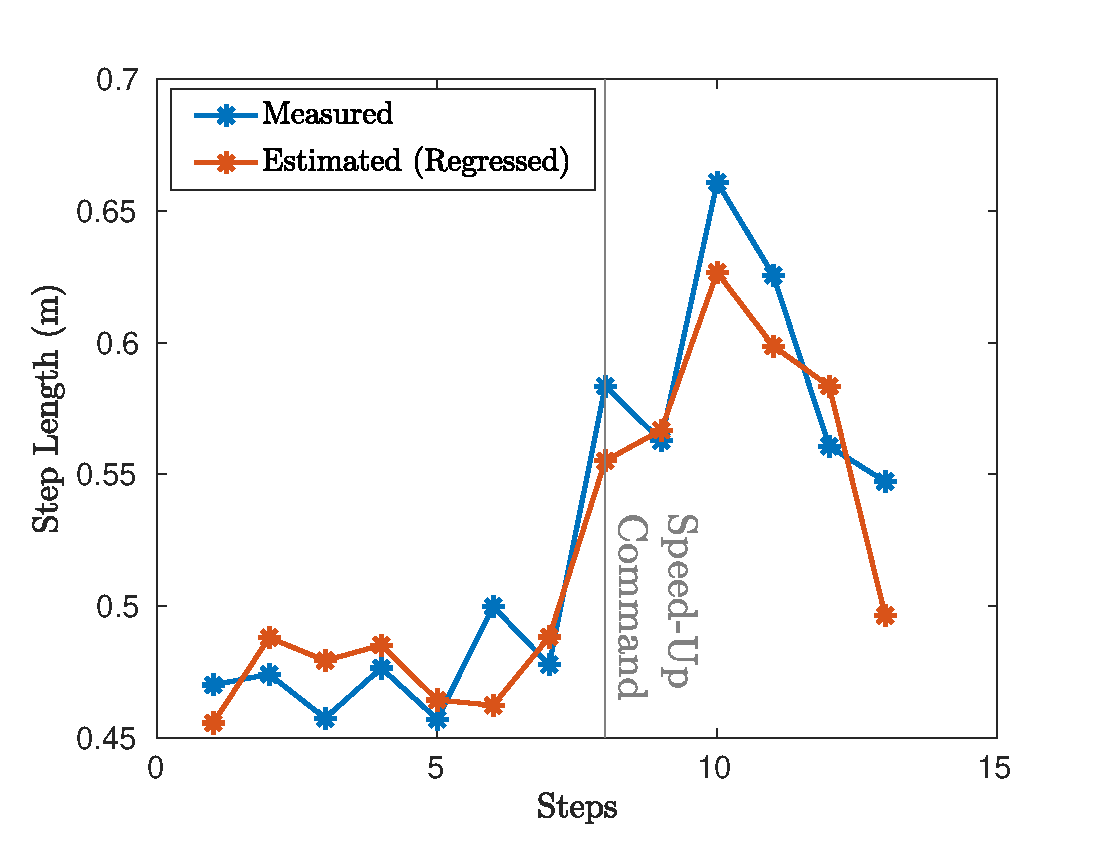
\includegraphics[width=0.7\linewidth]{ab_regress.eps}
	\caption{Performance of the regressed model, \eqref{eq:stepModel}, for the uninjured subject for a speed-up trial} \label{fig:ab_regressor}
\end{figure}

\begin{figure}
	\centering
	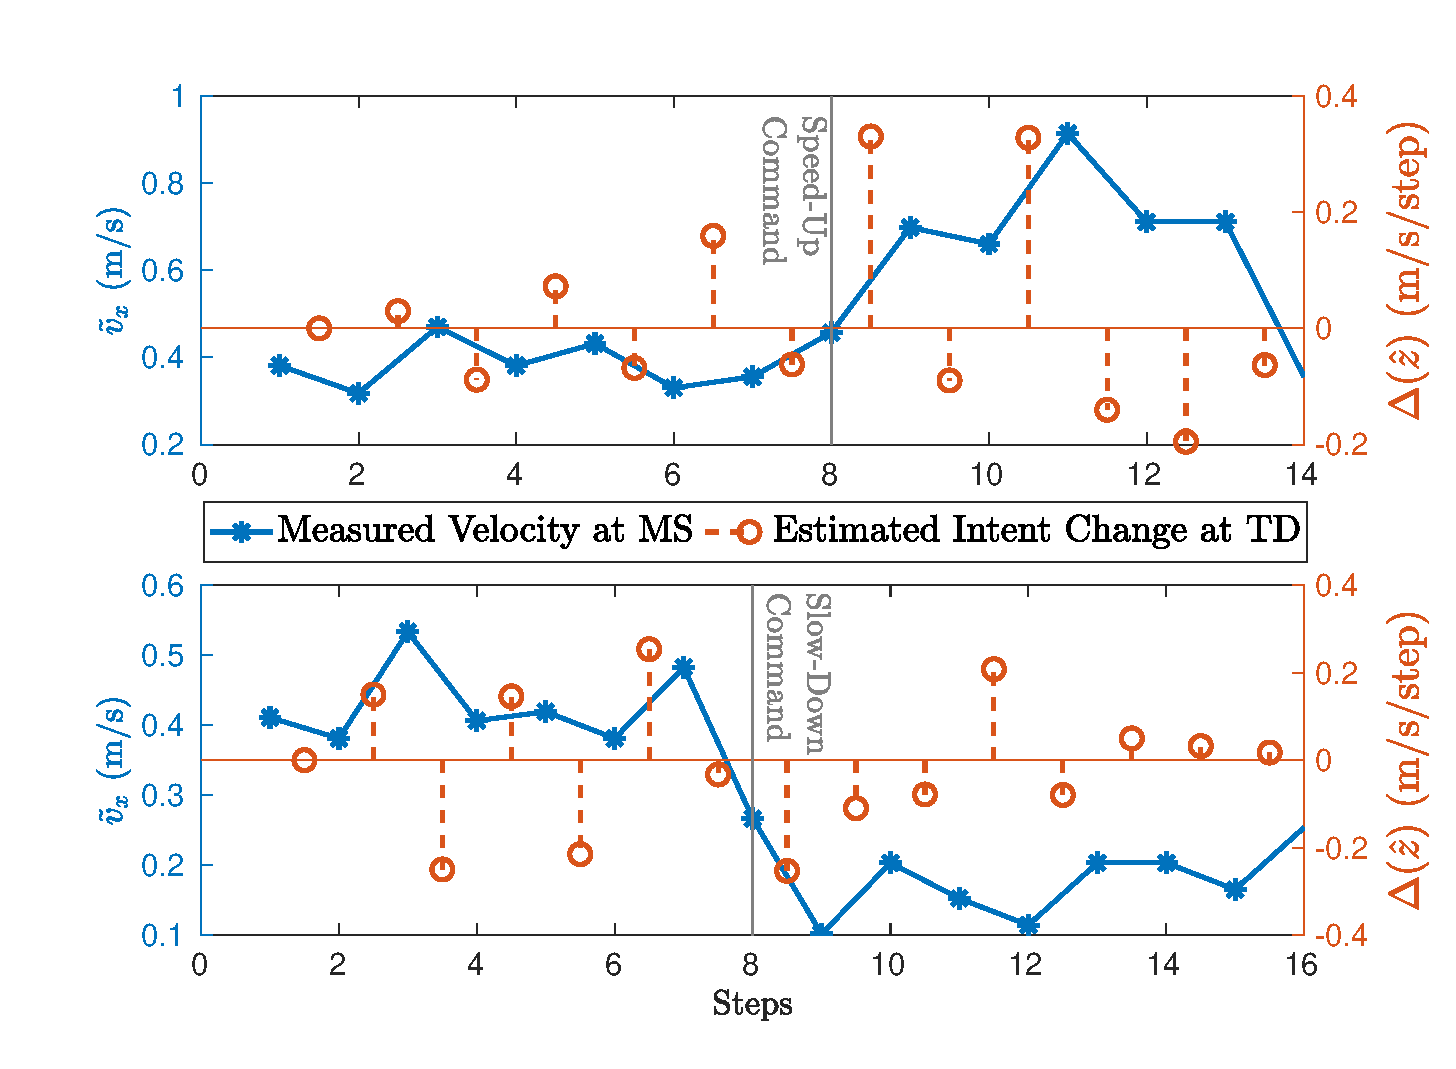
\includegraphics[width=0.7\linewidth]{ab_results.eps}
	\caption{Estimator performance for SU and SD trials for an uninjured subject} \label{fig:ab_results}
\end{figure}

The regression coefficients for the footstep model were $ \greekmat{\kappa} = [0.3325 ,0.2635 ,0.3757]^{\top} $ for this subject, with the units s, s, and m, respectively. The step lengths for an SU trial are shown in Fig.~\ref{fig:ab_regressor}. The regressed model was able to estimate the footstep to within $ \sim $ 5cm with an RMS error of 2.5cm. Consequently, it will be observed that footstep changes alone provided sufficient information to estimate intent changes in this case. The data in Fig.~\ref{fig:ab_results} illustrates the estimator performance for this trial. The stem plot represents the intent of the user as inferred at TD; a positive value indicates speed-up, and a negative value indicates slow-down anticipated for the subsequent MS. The vertical line represents the MS closest to the time the speed-change command was issued, and a significant speed change is to be expected after this step. The estimator accurately estimated the speed change for the trials, i.e., the value of the signal in the stem plot should be positive for speed-up and negative for slow-down after the command is issued.

The estimator performance for all trials of this subject is aggregated in Table.~\ref{table:ab_results_ag}. The ``Command Step" column refers to the MS when the command was issued, and the ``Detection Step" refers to the step during which TD the intent change was detected. Since the user must first process the command given, an intent detection delay of up to one step was deemed permissible. All SU and SD trials fit this criterion. 
%
\begin{table}[tb]
		\centering
		\caption{Speed change detection performance for trials with an uninjured subject} \label{table:ab_results_ag}
		\small
		\begin{tabular}{|c|c|c|}
			\hline 
		Trial	& Command Step & Detection Step \\ 
			\hline 
		SU - 01	& 8 & 8 \\ 
			\hline 
		SU - 02	& 8 & 8 \\ 
			\hline 
		SU - 03	& 8 & 9 \\ 
			\hline 
		SD - 01	& 7 & 7 \\ 
			\hline 
		SD - 02	& 7 & 7 \\ 
			\hline 
		SD - 03	& 7 & 7 \\ 
			\hline 
		\end{tabular} 
\end{table}%
%		
For further analysis, the estimated change in $ z $ for every step was compared to the measured change. If the speed change sign was correctly anticipated, it was considered a successful trial. The probability of successful intent change inference for the aggregated trials of the uninjured subject was 69\%, with a 95\% confidence interval \cite{brown2001interval} of 59\% - 78\%. The estimator has difficulty estimating intent changes when the velocity change is low, i.e., less than $ \sim $ 0.15 m/s due to insufficient changes in step lengths. This was the reason for a majority of the erroneous estimates, as the probability of success for this user increased to 95\%, with a confidence interval of 81\% to 100\%, when the steps with a measured speed change of less than 0.15 m/s were ignored.


\subsection{Subject with iSCI}\label{sec:nab_results}

The following evaluation uses data from trials of IU-2 (Sec.~\ref{sec:exoData}) who had previously experienced an incomplete SCI from the middle to the lower spine (T8 to L2). Individuals with these injuries generally exhibit good upper-body movement, control, and balance, but signals to the hips and legs are affected \cite{reevespinal}. % Had to cite Superman
For use with such an injury, the exoskeleton was set to adaptive mode. In this mode, the exoskeleton joints follow predefined trajectories and correct any deviations from them. Consequently, intent change is perceived as a deviation from the preset trajectories, and therefore, the exoskeleton attempts to correct the user's gait. 

The nature of the assistance provided in adaptive mode results in a difference in the goals of the user and the robot after the intent change. As a result, the step lengths did not exhibit significant enough variation or a consistent trend to allow for intent inference by themselves. The lack of step length variation is further supported by the regression coefficients for this subject $ \greekmat{\kappa} = [0.0818	,0.0551	,0.4045]^{\top} $, with the units s, s, and m, respectively. When compared to the regression coefficients for the model for the uninjured user, the iSCI model regression coefficients for $ v_k $ and $ (z-v_x)$ are smaller by an order of magnitude. This difference in coefficient magnitude shows there was not enough correlation between velocity changes and step length.

Figure~\ref{fig:nab_regressor} shows the step lengths for an SU trial; the estimated step lengths do not follow measurements, and only vary by $ \sim $2 cm throughout the trial, whereas the measurements vary by $ \sim $7 cm. Therefore, it was not possible to rely solely on footstep data.  Thus, the RMS current of the hip motor during the swing phase was added to the measurements obtained at TD, so that $ \tilde{\y}_{T} = [l_{step} ,I_{RMS}]^{\top} $. Another regression was performed to establish a relationship between the intended velocities and swing current:
\begin{equation}
	I_{RMS} = [v_x\ (z-v_x)] \greekvec{\alpha} \label{eq:currentModel},
\end{equation}
where $ \greekvec{\alpha} $ is a vector of the regression coefficients with units amperes-second per meter (As/m), found as $ \greekvec{\alpha} = [8.6067 ,4.2420]^{\top} $ for this trial. The process noise covariance $ \Q $  and the measurement noise covariance $ \R $ were then selected as follows.
\begin{eqnarray}
	\Q_M &=& {\rm diag}([1 ,1 ,1 ,1 ,1 ,1 ,10]) \times 10^{-4} \\
	\R_M &=& {\rm diag}([10^{4} ,10^{4} ,10^{4} ,10^{5} ,1 ,1]) \times 10^{-10} \\ % x y z vx vy vz at MS 
	\Q_T &=& 10^{-3}\\
	\R_T &=& {\rm diag}([1 ,1]) \times 10^{-4} % xf at TD
\end{eqnarray}
where noise covariances for positions, velocities, and currents are reported with units m\textsuperscript{2}, m\textsuperscript{2}/s\textsuperscript{2}, and A\textsuperscript{2}, respectively.

\begin{figure}
	\centering
	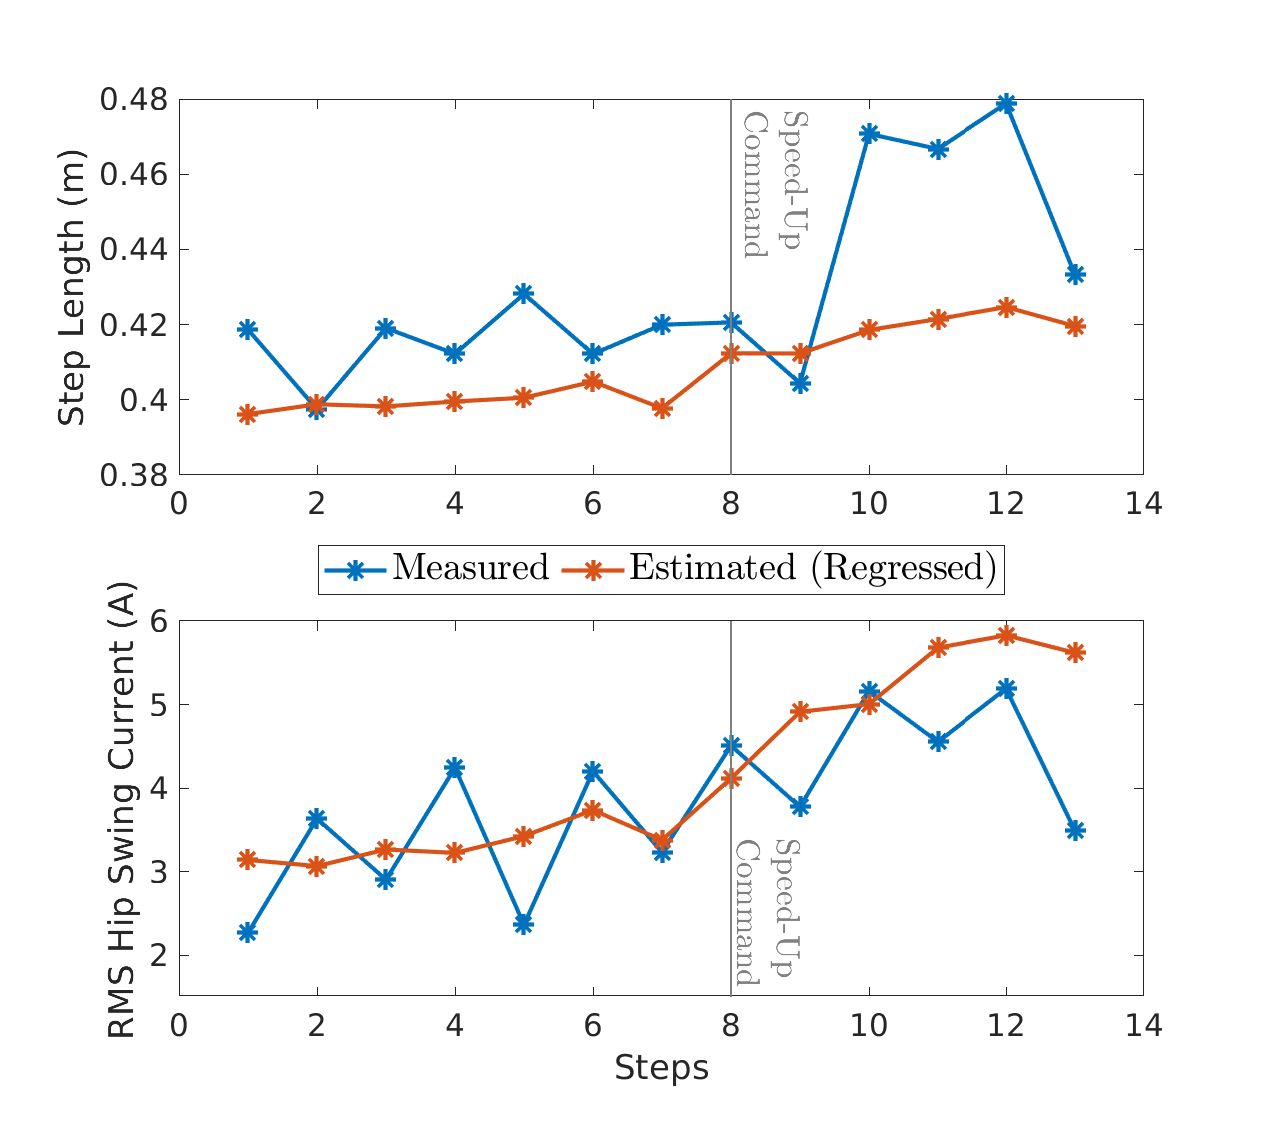
\includegraphics[width=0.72\linewidth]{nab_regress.eps}
	\vspace{-1em}
	\caption{Performance of the regressed models, Eqs.~\eqref{eq:stepModel} and \eqref{eq:currentModel}, for a subject with iSCI} \label{fig:nab_regressor}
\end{figure}


The hip current, in addition to the footstep data, provided sufficient information to be able to infer the user's intent immediately after the speed-change command was issued. The performance of the estimator for one of the SU trials with and without hip current measurements is illustrated in Fig.~\ref{fig:c_v_f}. 

\begin{figure}
	\centering
	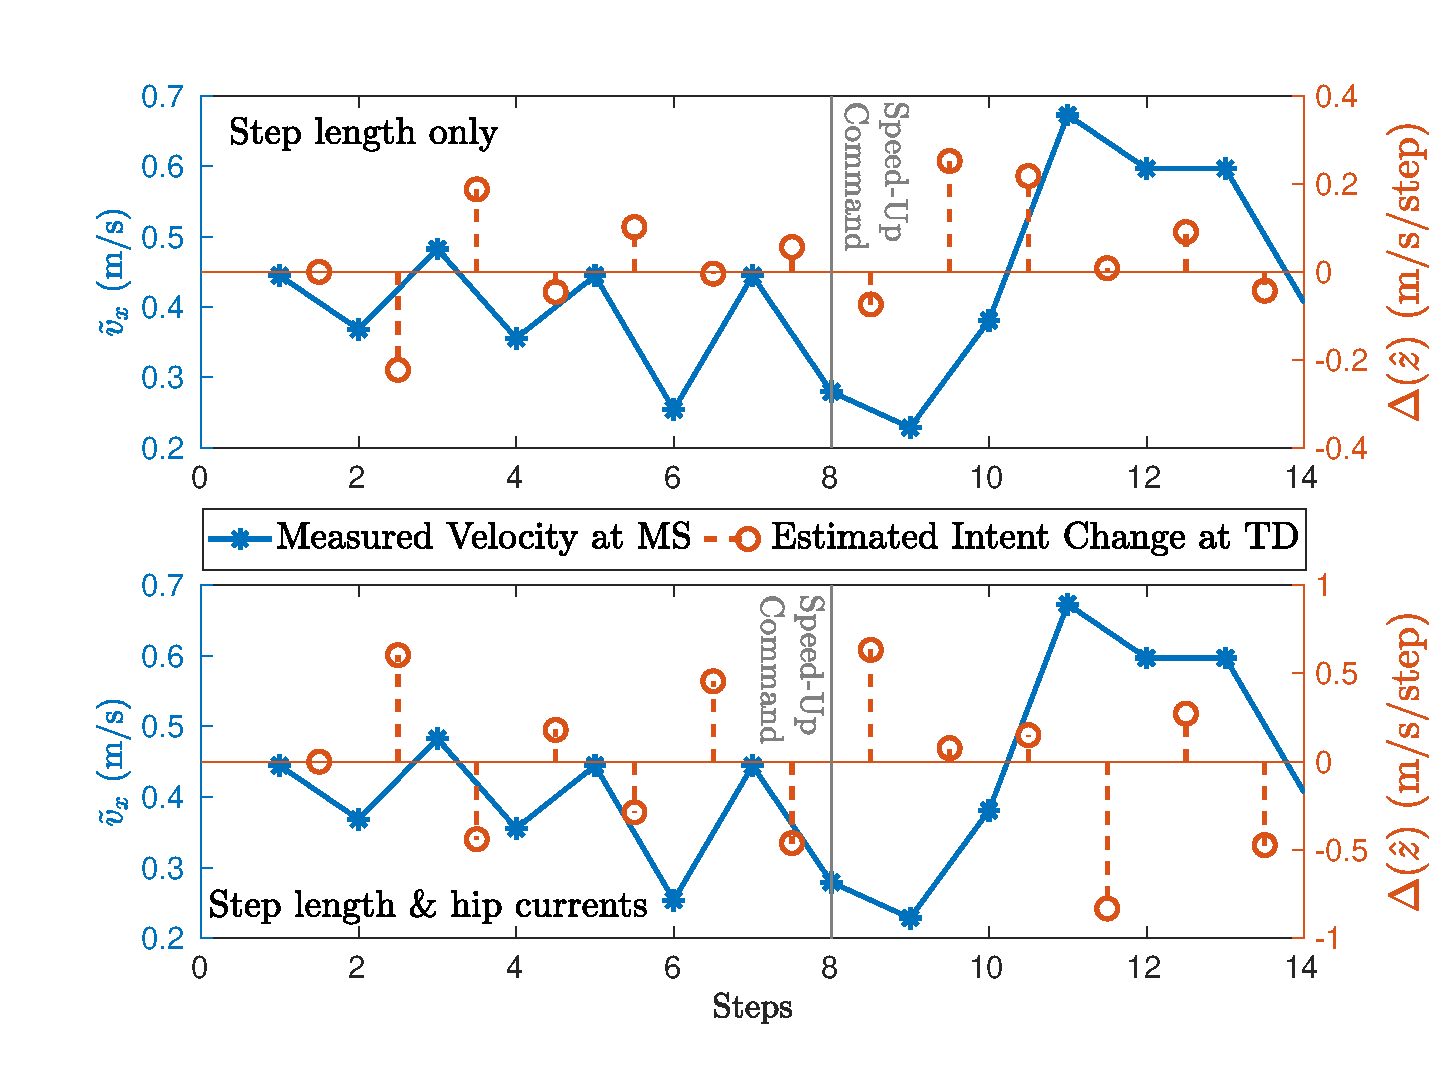
\includegraphics[width=0.75\linewidth]{curr_v_footsteps.eps}
	\vspace{-1em}
	\caption{Estimator performance comparison before and after including hip current measurements} \label{fig:c_v_f}
\end{figure}

When relying solely on step length measurements, the estimator was unable to output accurate speed-up/slow-down signals in the beginning of the trial, and the change in intent to speed up was detected a step after the command was issued. There was a small dip of 0.05 m/s in velocity after the speed up command was issued, and this may be because the exoskeleton assistance in adaptive mode overpowered the user's motion in order to maintain the nominal joint trajectory. However, with the inclusion of hip motor currents, the estimator was able to correctly identify the intent to speed up during the same step the command was issued and before the user began physically speeding up. This anticipative performance of the estimator is shown in Fig.~\ref{fig:nab_results} for additional SU and SD trials.
 
\begin{figure}
	\centering
	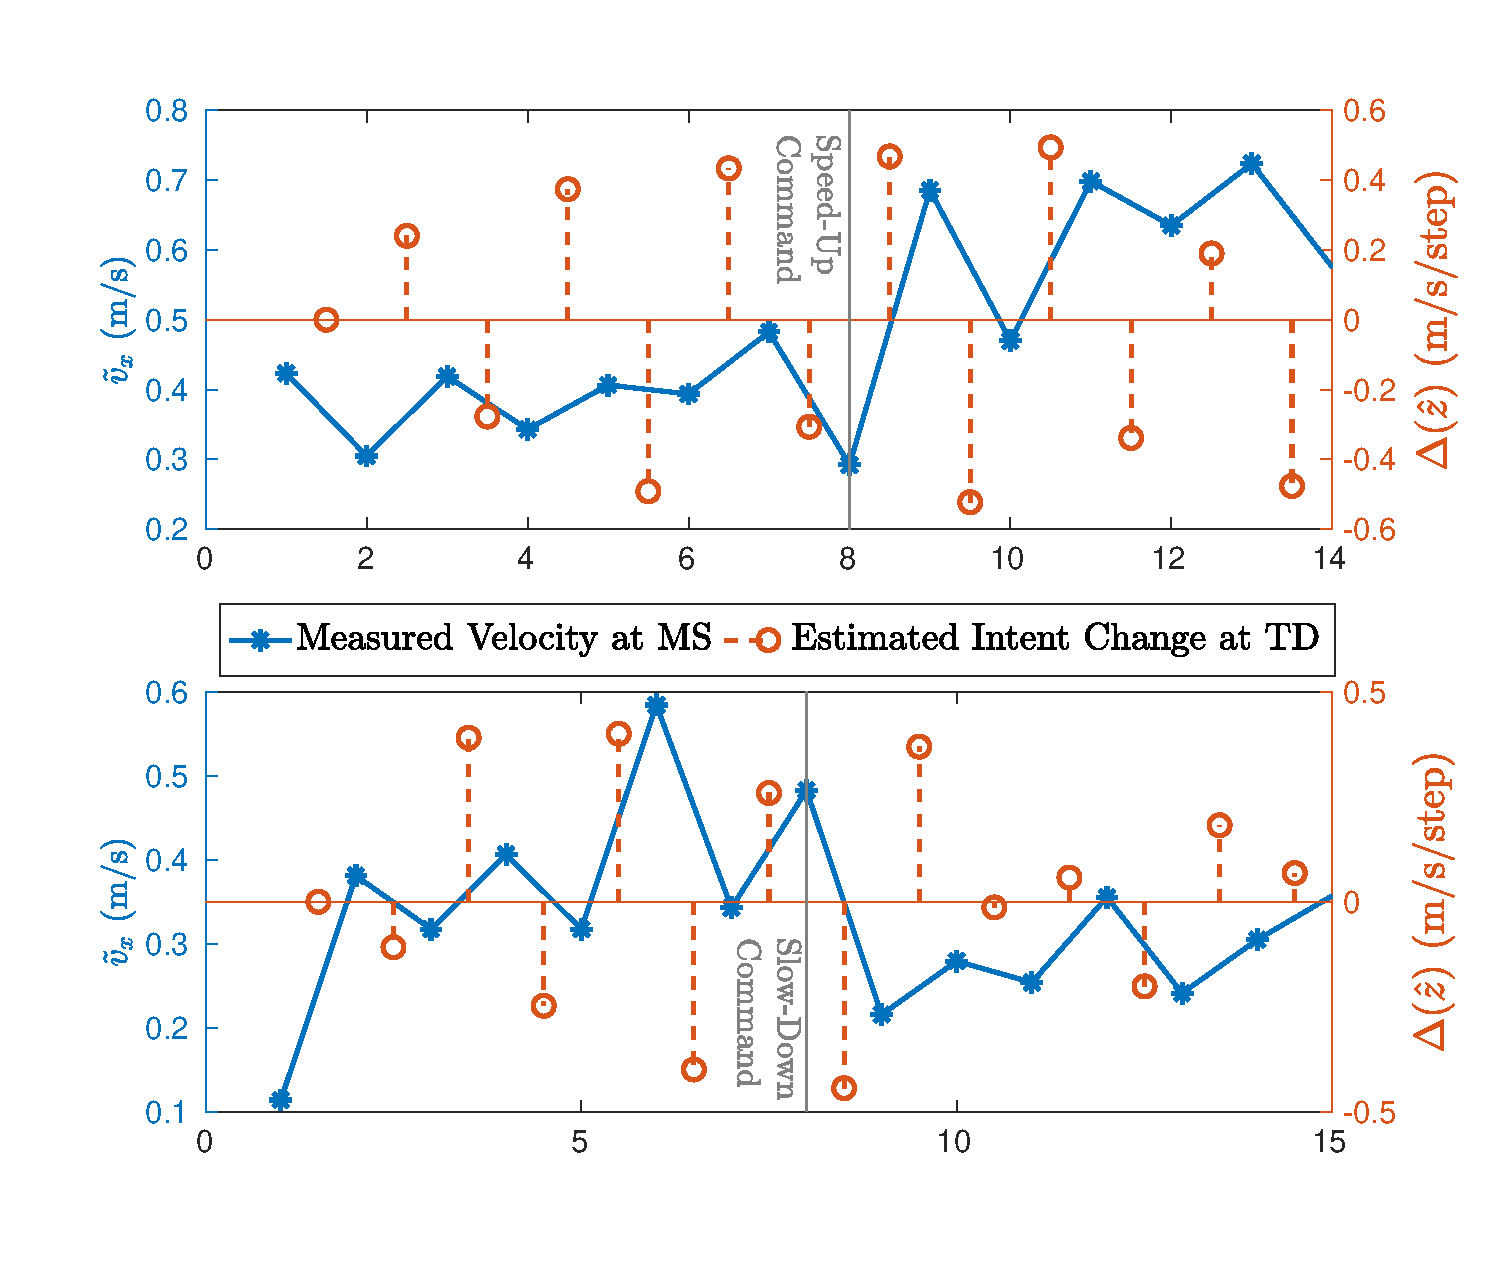
\includegraphics[width=0.7\linewidth]{nab_results.eps}
	\caption{Estimator performance for SU and SD trials for a subject with iSCI} \label{fig:nab_results}
	\vspace{-1em}
\end{figure}

The estimated value of $ \hat{z} $ for one SU trial was compared to the measured forward velocity over the trial, as illustrated in Fig.~\ref{fig:m_v_e}. The vertical solid lines denote MS, and red stars denote the value of $ \hat{z} $, i.e., the estimate of the user's intended velocity. Since $\hat{z}$ represents the desired speed of the user, its value at TD was compared to the measured velocity at the subsequent MS, by which point the intended velocity should be realized. Therefore, by comparing the position of a red star with the preceding star, the estimator output can be interpreted as a speed-up change if a star is higher, and a slow-down change if it is lower. As $ \hat{z} $ is estimated at TD, the red stars are indicative of future trends. The values of $ \hat{z} $ show strong correlation with the measured values of $v_x$ at the next MS, but are not exact. For the trial illustrated in Fig.~\ref{fig:m_v_e}, the correlation coefficient of $ \hat{z} $ at TD to the measured $ v_x $ at the next MS was 0.63. By comparison, the correlation coefficient of $ \hat{v}_x $ at TD to the measured $ v_x $ at the next MS was -0.11. This correlation further bolsters the hypothesis that incorporating information at touchdown in the estimator is valuable for anticipating speed changes.

\begin{figure}
	\centering
	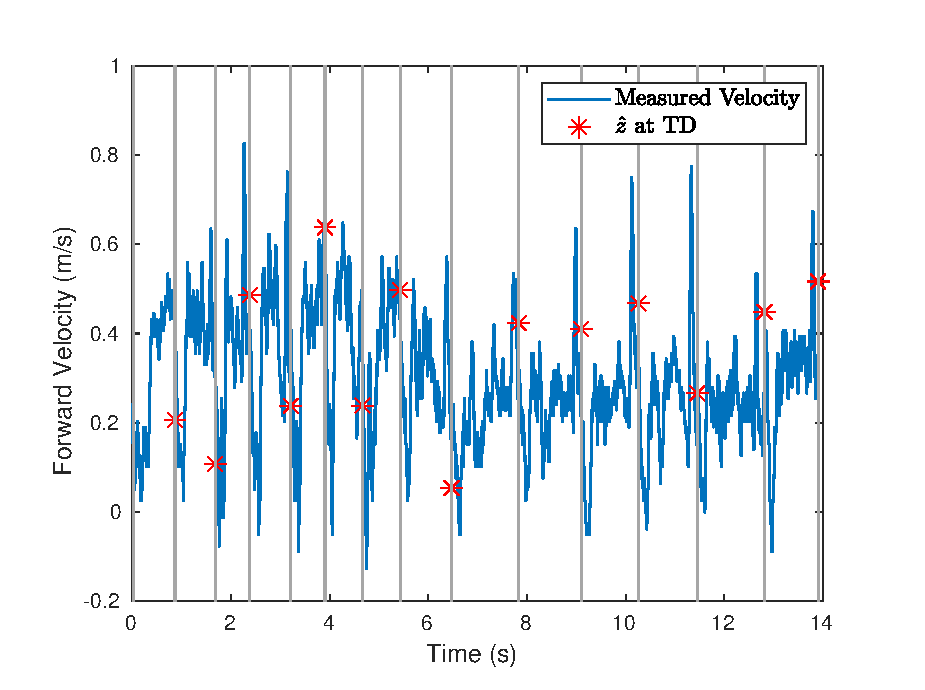
\includegraphics[width=0.8\linewidth]{estimated_vs_measured.eps}
	\caption{Estimated desired velocity at MS as predicted at TD ($\hat{z}$) compared to velocity $v_x$ over the stride.} \label{fig:m_v_e}
\end{figure}

The estimator performance for all trials of this subject is aggregated in Table~\ref{table:nab_results_ag} with similar pass/fail criteria as the trials with the uninjured subject. For trial SD-03, the estimator detected the speed change after the command, but there were estimator inaccuracies for the subsequent step. There were fluctuations of $ \sim $0.15~m/s in the forward velocity of the user after the command was issued. This may be due to the high gait variability due to spastic disturbances that are common in individuals with SCIs \cite{malhotra2009spasticity}. It has been observed that it is more difficult to detect speed-up intent changes in injured individuals since the intent signal is considerably diminished compared to slow-down trials \cite{gambon2020effects} due to the user's reduced strength.

\begin{table}[tb]
		\centering
		\caption{Speed change detection performance for trials with a subject with an iSCI} \label{table:nab_results_ag}
		\small
		\begin{tabular}{|c|c|c|c|c|}
			\hline 
			Trial	& Command Step & Detection Step \\ 
			\hline 
			SU - 01	& 8 & 8 \\ 
			\hline 
			SU - 02	& 8 & 8 \\ 
			\hline 
			SU - 03	& 7 & 11 \\ 
			\hline 
			SD - 01	& 8 & 8 \\ 
			\hline 
			SD - 02	& 7 & 7 \\ 
			\hline 
			SD - 03	& 8 & 8 \\ 
			\hline 
		\end{tabular} 
\end{table}

The aggregate probability of success for walking trials of the subject with iSCIs was 78\% with a 95\% confidence interval of 68\% to 86\%. All trials except SD-03 had individual percentages of success of at least 70\%. Trial SU-02 had a probability of success of 92\%, and SU-01 and SD-01 had a 100\% success rate. It is worth noting that the trials with high success rates were performed when the subject was rested, and SD-03 was the last of multiple back-to-back trials. The subject's exhaustion may have diminished their ability to resist the exoskeleton's inputs and therefore, made intent estimation difficult.

The estimator uses simple dynamics that do not use knowledge of legged locomotion. These simple dynamics along with the limited data to generate the footstep model result in the framework only being able to identify whether the user wants to speed up or slow down and not the target velocity the user wishes to reach. This behavior may be remedied with strategies that establish a more precise relationship between intended gait speed and gait features such as foot placement, and motor currents. The scarcity of training data and revisions to the models that relate gait speed and gait features are addressed in Chapter~\ref{chapter:MP}.

\section{Exploring the effects of increasing the number of considered gait features and model complexity on estimator accuracy}\label{sec:add_analysis}

Two possible strategies were considered to increase estimator accuracy in detecting SU/SD changes and predicting the magnitude of the desired velocity. One strategy was to increase the number of gait features considered at TD. The other was to replace the simple linear models with more complex models such as polynomial models or Gaussian Process Regression (GPR) models. Estimator performance was evaluated primarily using the probability of success. However, another metric considered was the root mean square (RMS) error between the predicted gait speed change at TD and the value measured at the subsequent MS. The following analysis was only performed on data from an uninjured user walking in free mode using a walker, as it was hypothesized that a strong correlation between gait speed and gait patterns existed for this user. The estimator configurations considered for this analysis are detailed as follows. Section~\ref{sec:increase_meas} describes the selection of step frequency as the additional measurement. Sections~\ref{sec:linear},~\ref{sec:poly}, and~\ref{sec:GPR} describe estimation performance when using linear, polynomial, and GPR models, respectively. The conclusion of this analysis is provided in Section~\ref{sec:analysis_conc}
%
%\begin{table} %SU
%	\centering
%	\caption{Estimator performance of all configurations for only SU trials} \label{table:su}
%	\small
%	\begin{tabular}{|c|c|c|c|}
%		\hline
%		Model & No. of meas. & Probability of success (\%) & RMS error (m/s)\\
%		\hline
%		Linear & 1 & 79 & 0.15 \\
%		\hline
%		Linear & 2 & 82 & 0.12 \\
%		\hline
%		Polynomial & 1 & 61 & 0.14 \\
%		\hline
%		Polynomial & 2 & 76 & 0.12 \\
%		\hline
%		GPR & 1 & 47 & 0.15 \\
%		\hline
%		GPR & 2 & 51 & 0.15 \\
%		\hline
%	\end{tabular}
%\end{table}
%
%\begin{table} %SD
%	\centering
%	\caption{Estimator performance of all configurations for only SD trials} \label{table:sd}
%	\small
%	\begin{tabular}{|c|c|c|c|}
%		\hline
%		Model & No. of meas. & Probability of success (\%) & RMS error (m/s)\\
%		\hline
%		Linear & 1 & 61 & 0.13 \\
%		\hline
%		Linear & 2 & 63 & 0.16 \\
%		\hline
%		Polynomial & 1 & 61 & 0.09 \\
%		\hline
%		Polynomial & 2 & 53 & 0.18 \\
%		\hline
%		GPR & 1 & 79 & 0.09 \\
%		\hline
%		GPR & 2 & 79 & 0.08 \\
%		\hline
%	\end{tabular}
%\end{table}

\subsection{Increasing the number of measurements at touchdown}\label{sec:increase_meas}
Estimator configuration and the considered measurements have a significant impact on estimator performance. The configurations of the BKF presented in previously were able to anticipate changes in gait speed before they were realized. However, the estimator was not able to precisely estimate the magnitude of the anticipated velocity change. The estimator was configured to rely on only the step length for the trials with an uninjured user. Using measurements from more gait features during estimation may provide more information about the user's desired gait speed and be a possible solution to improve estimator performance.

The following analysis was conducted using data from walking trials of an uninjured user with the exoskeleton in free mode. The dataset of an uninjured user was chosen to minimize gait variability as users with iSCIs exhibit higher variability \cite{sohn2018variability}. There are two benefits of considering trials in free mode; gait patterns may reflect the coupling of human-robot dynamics and also exhibit low noise as the exoskeleton does not resist the user's motions. This choice of dataset may make the relationship between gait velocity and the indicators of intent more apparent during the analysis. 

Appropriate gait features must be chosen to prevent adding misleading measurements that may prove detrimental to estimator performance. Candidate gait features to include in the estimator were torso pitch and roll angles and angular velocities, and step frequency. As intent estimation happens midway through a step at TD, the step frequency was posed as the ``time-to-TD" ($ t_{TD} $) from MS. Upon comparison to forward velocity at MS, the angles and angular velocities of the torso did not show a significant correlation with gait velocity. This lack of correlation was further confirmed as the correlation coefficients of the torso angles were $ \approx $ 0.2 with p-values greater than 0.5, where the null hypothesis was that the quantities were uncorrelated. The lack of correlation may be explained by the lack of exoskeleton resistance to the user's motions. Torso angles and angular velocities may exhibit a correlation with gait speed in adaptive mode \cite{suzuki2007intention}. In contrast, $ t_{TD} $ and step length $ l_{step} $ were found to be highly correlated to gait velocity, with correlation coefficients greater than 0.7 and p-values less than 0.05. Therefore, $ t_{TD} $ and $ l_{step} $ were chosen for inclusion in the estimator. It is challenging to manually select additional gait features, and methods to automate this process and deal with user-specific feature relevance are discussed in Chapter~\ref{chapter:MP}.

Similarly to the process described in Section~\ref{sec:bkf_results}, a dataset was created for these gait features from a set of 3 SU and SD trials each. The regressions were set up such that $ \Psi_{k+1} = f(v_k,z_k) $, where $ \Psi $ was the gait feature to be modeled.

\subsection{Estimation using linear models}\label{sec:linear}

The estimator trials of the uninjured user with measurements of step length at TD (Section~\ref{sec:ab_results}) were used to establish a baseline. The percentage of successful inference of the user's desire to change velocity for every step in the aggregated trials of the uninjured subject was 70\% with a 95\% confidence interval of 60\% - 79\%. Step length was modeled as described in \eqref{eq:stepModel}. A second model $t_{TD} =  [v_x\ (z - v_x)\ 1] \greekvec{\xi}_{lin}$ was used to establish a relationship between velocity and step frequency, where $ \greekvec{\xi}_{lin} $ was calculated similarly to the step length model. This model for $ t_{TD} $ differs from \eqref{eq:stepModel} as $ l_{leg} $ was used as the constant when modeling step length. The RMS regression error for this model was 0.12s. The values of $ \greekvec{\kappa}_{lin} $ and $ \greekvec{\xi}_{lin} $ were $[0.34 ,0.37 ,0.37]^T$ and $ [-0.45 ,-0.48 ,0.64]^T $, respectively. The coefficients contained in $ \greekvec{\kappa}_{lin} $ have the units s, s, and m, and the coefficients in $ \greekvec{\xi}_{lin} $ have the units s\textsuperscript{2}/m, s\textsuperscript{2}/m, and s, respectively.

The estimator with two measurements was rerun for all trials and consistently had success rates greater than 75\% for SU trials and less than 70\% for SD trials except one, which had a 78\% success rate. Compared to the baseline, the aggregated success rate for all trials increased from 69\% to  72\% with a 95\% confidence interval~\cite{brown2001interval} of 62\% - 81\%, and the aggregate RMS error between the estimated and measured gait speed increased from 0.14 m/s to 0.142 m/s. The aggregate estimator performance for SU and SD trials is listed in Table~\ref{table:linear}. Performance improvements were seen for both SU and SD trials when using two measurements. The next step was to explore the effects of increasing model complexity on the RMS error and speed change detection accuracy with two candidate model types, polynomial and GPR.

\begin{table}
	\caption{Estimator performance of all configurations with linear models - SU/SD trials} \label{table:linear}
	\centering
	\begin{tabularx}{\linewidth}{|C|C|C|C|C|}
	\hhline{-----}
	\multicolumn{1}{|c|}{}  & \multicolumn{2}{c|}{Probability of Success (\%)} & \multicolumn{2}{c|}{RMS error (m/s)} \\
	\hhline{-----}
	No. of meas. & SU & SD & SU & SD \\
	\hhline{-----}
	1	& 79 & 61 & 0.15 & 0.13 \\
	\hline
	2	& 82 & 63 & 0.12 &  0.16 \\
	\hhline{-----}
	\end{tabularx}
\end{table}

\subsection{Estimation using polynomial models}\label{sec:poly}

Model complexity was increased to try and establish a more comprehensive relationship between the velocity and gait features. Since experimental data have shown the stride frequency and step length relationship to be proportional to the square of the gait velocity~\cite{bailey2017relationship}, second-degree polynomials were considered to model $ l_{step} $ and $ t_{TD} $ as functions of $ v_x $ and $ z $. The models had a general structure $ \Psi = [1\ a\ b\ a^2\ ab\ b^2 ] \greekvec{\lambda}$, where $ \Psi $ represents the gait feature, $ l_{step} $ or $ t_{TD} $, $ \greekvec{\lambda} $ represents a vector of the regression coefficients $ \greekvec{\kappa}_{poly} $ or $ \greekvec{\xi}_{poly} $, and $ a $ and $ b $ represent $v_x$ and $(z - v_x) $, respectively. Compared to the linear model with one measurement, the aggregated success rate for all trials decreased from  69\% from 64\% with a 95\% confidence interval of \mbox{53\% - 75\%}, while the aggregate RMS error decreased from 0.14 m/s to 0.12 m/s. The aggregate estimator performance for SU and SD trials is listed in Table~\ref{table:poly}, and in this case, the performance for SD trials decreased when $ t_{TD} $ was included.

\begin{table}
	\caption{Estimator performance of all configurations with polynomial models - SU/SD trials} \label{table:poly}
	\centering
	\begin{tabularx}{\linewidth}{|C|C|C|C|C|}
		\hhline{-----}
		\multicolumn{1}{|c|}{}  & \multicolumn{2}{c|}{Probability of Success (\%)} & \multicolumn{2}{c|}{RMS error (m/s)} \\
		\hhline{-----}
		No. of meas. & SU & SD & SU & SD \\
		\hhline{-----}
		1	& 61 & 61 & 0.14 & 0.09 \\
		\hline
		2	& 76 & 53 & 0.12 &  0.18 \\
		\hhline{-----}
	\end{tabularx}
\end{table}

\subsection{Estimation using Gaussian Process Regression}\label{sec:GPR}

The second class of models considered for this comparison was Gaussian Processes (GPs) to try and capture complex relationships between gait features. A GP is a set of random variables, such that any finite number of them have a joint Gaussian distribution \cite{rasmussen2006gaussian}. The mean of this distribution is generally assumed to be zero, and the covariance is given by the kernel function. This function gives the covariance between two random variables at two points in time, and its performance is tuned using certain hyperparameters. Changing these hyperparameters affects the smoothness of the functions that can be sampled from the GP.

For Gaussian Process Regression (GPR), let $ \vec{y} \in \mathbb{R}^n $ be a vector of $ n $ observations and $ \vec{x} \in \mathbb{R}^n  $ be the corresponding input vector. Let $ \vec{x}_{*} \in \mathbb{R}^m$ be the test points for prediction. The first step when predicting the response variable $ \vec{y}_{*} $ at $ \vec{x}_{*} $ is to form a joint prior distribution of the training and test data. 
\[
	\begin{bmatrix}
		\y \\
		\y_{*}
	\end{bmatrix} \sim \mathcal{N} \left(\mathbf{0},%
	\begin{bmatrix}
		K(\x,\x) & K(\x,\x_{*}) \\
		K(\x_{*},\x) & K(\x_{*},\x_{*})
	\end{bmatrix}\right)
\]
where $ K $ is a matrix formed by evaluating the kernel function for all training and test data. The response of the GP can then be modeled as the probability of $ \y_{*} $ conditioned on $ \x $, $ \y $, and $ \x_{*} $, i.e., $ p(\y_{*}|\x,\y,\x_{*}) $. Furthermore, basis functions can be included to model the response variable
\[
	\y_{*} = f(\vec{x}_{*}) + h(\vec{x}_{*})^T \greekvec{\beta}
\]
where $ f(\vec{x}_{*}) \sim \mathcal{GP}(\mathbf{0},K(X,X_{*})) $, $ h(\vec{x}_*) $ is an optional basis function, and $ \greekvec{\beta} $ is a vector of coefficients. While this presentation serves as a brief introduction to GPs, the interested reader is referred to~\cite{rasmussen2006gaussian}.
%The Gaussian Process Regression (GPR) may then be formulated with a GP $ f(\vec{x}_{*}) \sim \mathcal{GP}(0,k(\vec{x},\vec{x}_{*})) $ where $ k(\vec{x},\vec{x}_{*}) $ is the kernel evaluated at a test point. 
%Furthermore, an optional basis function $ h(\vec{x}) $ with coefficients $ \greekvec{\beta} $ may be added
%\begin{equation}
%	\y_{*} = h(\vec{x}_{*})^T \greekvec{\beta} + f(\vec{x}_{*})
%\end{equation}
%This inclusion of the basis function implies the data is close to the basis function and the residuals can be modeled by the GP making GPRs probabilistic and nonparametric. %While the current presentation aims to be self contained, the interested reader is referred to \cite{rasmussen2006gaussian,mackay2003information}.

Regression was performed on measurements to fit the GP models for $ l_{step} $ and $ t_{TD} $ using the \texttt{fitrgp} function in  MATLAB. This function maximizes the log likelihood function using Bayesian optimization to select values of $ \greekvec{\beta} $, the kernel, and associated hyperparameters to best fit the training data. The GPR model for $ l_{step} $ was a function of $ v_x $, $ z-v_x $ and $ l_{leg} $ using the Rational Quadratic kernel 
\begin{align*}
	k(x,x_*) &= \sigma_f^2 \left( 1 + \frac{r^2}{2 \alpha \sigma_l^2}\right)^{-\alpha}\\
	r &= \sqrt{(x-x_*)^T(x-x_*)}
\end{align*}
where the hyperparameters $ \sigma_f $, $ \sigma_l $, and $ \alpha $ are the signal standard deviation, length-scale, and a scale-mixture parameter, respectively. Length-scale is a measure of the distance between two input values that may cause response values to become uncorrelated. Too small a length-scale may result in overfitting, and a large length-scale may result in a poor fit. The values of $ \sigma_f $, $ \sigma_l $, and $ \alpha $ were 0.04, 0.08, and 4.19$ \times $10\textsuperscript{4}, respectively, and the basis function was quadratic.

The GPR model for $ t_{TD} $ was a function of $ v_x $ and $ z-v_x $ using a variation of the Squared Exponential kernel  
\[
	k(x,x_*) = \sigma_f^2 exp\left[-\frac{1}{2} \displaystyle \sum_{m = 1}^{d} \frac{(x_m - x_{*m})^2}{\sigma_m^2} \right]
\]
In this variation, each predictor, $ v_x $ and $ z-v_x $, has a different length scale. These length scales are collected in $ \greekvec{\sigma}_m \in \mathbb{R}^{d \times 1}$, where $ d $ is the number of predictors. The values for $ \sigma_f $, $ \sigma_1 $, and $ \sigma_2 $ were 0.44, 5.97, and 16.15, respectively and no basis function was chosen for the GPR model for $ t_{TD} $.  
%
%Hyperparameters are the free parameters in a kernel such as signal standard deviation $ \sigma_f $ and length-scale $ \sigma_l $. Input point may have different length-scales, collected in $ \greekvec{\sigma}_m \in \mathbb{R}^{d \times 1}$ where $ d $ is the number of input points. 
%
%\begin{table}
%	\centering
%	\caption{Kernels used in GPR models}\label{table:kernel}
%	\begin{tabular}{|c|c|}
%		\hline
%		Rational Quadratic & ARD Squared Exponential \\
%		\hline
%		{$\begin{aligned}
%				k(x,x_*) &= \sigma_f^2 \left( 1 + \frac{r^2}{2 \alpha \sigma_l^2}\right)^{-\alpha}\\
%				r &= \sqrt{(x-x_*)^T(x-x_*)}
%			\end{aligned}$} & $ k(x,x_*) = \sigma_f^2 exp\left[-\frac{1}{2} \displaystyle \sum_{m = 1}^{d} \frac{(x_m - x_{*m})^2}{\sigma_m^2} \right] $ \\
%		\hline
%	\end{tabular}
%\end{table}

As listed in \eqref{eq:tdUp} and \eqref{eq:tdCovUp}, the BKF framework needs a Jacobian of the measurement models to perform the Bayesian update at TD. It is possible to compute the Jacobians analytically for the GPR models; however, they were computed numerically via finite difference to allow changing models and to test different kernel functions without significant overhead. As GPR models are probabilistic, the uncertainty of their predictions is was computed and incorporated into the estimator. This inclusion was able to improve the estimation accuracy for the trials, and similar updates may not be performed with other model families due to the absence of a kernel function. Over all the SU and SD trials, this configuration had a success rate of 70\% with a confidence interval of 59\% to 79\% and an RMS estimation error of 0.12 m/s. This RMS error was the lowest of all the configurations. This configuration had an accuracy of 79\% for SD trials and 61\% for SU trials. The aggregate estimator performance for SU and SD trials is listed in Table~\ref{table:GP}, and improvements in estimator performance were seen for SU trials, but not for SD trials, when $ t_{TD} $ was included in the estimator.

\begin{table}
	\caption{Estimator performance of all configurations with Gaussian Process Regression models - SU/SD trials} \label{table:GP}
	\centering
	\begin{tabularx}{\linewidth}{|C|C|C|C|C|}
		\hhline{-----}
		\multicolumn{1}{|c|}{}  & \multicolumn{2}{c|}{Probability of Success (\%)} & \multicolumn{2}{c|}{RMS error (m/s)} \\
		\hhline{-----}
		No. of meas. & SU & SD & SU & SD \\
		\hhline{-----}
		1	& 47 & 79 & 0.15 & 0.09 \\
		\hline
		2	& 51 & 79 & 0.15 &  0.08 \\
		\hhline{-----}
	\end{tabularx}
\end{table}

\subsection{Conclusion: Increasing the number of gait features versus model complexity}\label{sec:analysis_conc}
In general, estimator configurations with two measurements, step length and step frequency, showed improvements in performance over its counterpart with one measurement. There was no clear superior configuration, as the estimator with the linear model and two measurements performed best for SD trials in terms of both probability of success and RMS error, while the GPR model performed best for SU trials. For both SU and SD trials combined, the linear model with two measurements had a success rate of 72\% and an RMS error of 0.15 m/s, whereas the GPR model had a success rate of 70\% with an RMS error of 0.12 m/s. It is important to note that these are aggregate results, and overall, configurations with two measurements had better accuracy than those with a single measurement. In contrast, increasing  model complexity did not yield significant improvements in estimator accuracy, but resulted in an increased number of parameters that require tuning. This tuning problem will get increasingly challenging as more gait features are considered. Therefore, the number of gait features considered in the work presented in Chapter~\ref{chapter:MP}, was increased to 18 to better exploit pHRI in the estimation framework.

\section{Summary}\label{sec:bkf_summary}

This chapter showed that the intent detection framework based on a Buttressed Kalman Filter is capable of predicting intent changes in exoskeleton users with and without iSCIs based on foot placement and leg swing currents. It can be inferred that the hip currents may be a better indicator of intent in individuals with iSCIs, as their actions to modify their foot placement may not be completed due to the resistance from the exoskeleton. So it can be argued that attempted foot placement is the primary mechanism of exhibiting intent change in individuals with iSCIs, but the human-robot interface causes this information to show up on hip current rather than kinematic data. This result motivated the consideration of measurements from multiple gait features at TD.

Including additional measurements at TD had a larger contribution toward increasing the estimator's probability of success than did increasing the complexity of the measurement models. Neither of these two approaches had a conclusive effect on increasing the metric precision of the estimated desired speed. The estimator had difficulty using gait features to detect speed changes under 0.15 m/s, often leading to false predictions and leading to deterioration in estimator accuracy. These false predictions were confirmed, when steps with a measured speed change of less than 0.15 m/s were ignored during estimation trials of the uninjured user. The probability of success increased from 69\% to 95\%. Thresholds based on a user's gait variability may be incorporated to reject these false predictions. As evidenced by the use of different gait features for subjects with and without iSCI, gait feature relevance may be user-specific, which motivates the personalization of estimators to maintain estimation accuracy, as is explored in the following chapter.